\section{Zielsetzung}
\label{sec:Zielsetzung}
Ziel dieses Versuches ist Untersuchung der Funktionsweise, sowie der charakteristischen
Parameter eines Geiger-Müller-Zählrohrs bei der Detektion von ionisierender Strahlung.

\section{Theorie}
\label{sec:Theorie}
Im Folgendem wird der grundlegende Aufbau eines Geiger-Müller-Zählrohrs, 
sowie die physikalischen Abläufe im Inneren und die Zählrohrcharakteristik erklärt.

\subsection{Aufbau und Funktionsweise eines Geiger-Müller-Zählrohrs}
\label{subsec:AufuFunk}
Das Geiger-Müller-Zählrohr wird verwendet um die Intensität ionisierender Strahlung
zu messen. Der Aufbau besteht aus einem Hohlzylinder mit dem Radius $r_A$, dessen Außenwand  als Kathode
dient, sowie einem Anodendraht mit dem Radius $r_k$ in der Mitte des Zylinders. Das Innere des Hohlzylinders
ist mit einem Gasgemisch gefüllt und unterliegt einem Unterdruck. Dies führt dazu, dass sich die dünnwandige
Mylar-Folie am Eintrittsfenster des Zählrohrs nach Innen wölbt. Der schematische Aufbau ist in \autoref{fig:Abb_1}
dargestellt.
\begin{figure}[H]
    \centering
    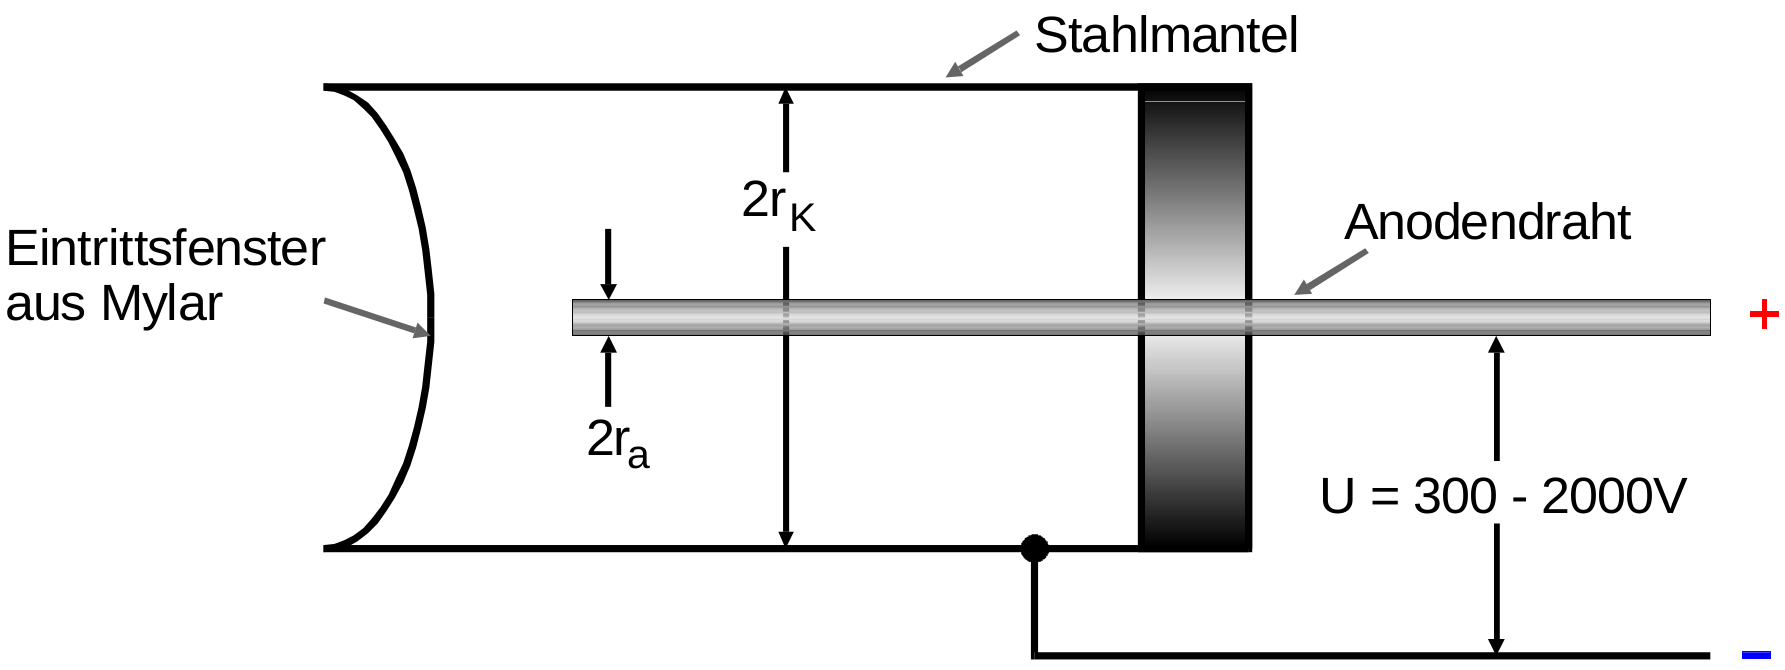
\includegraphics[width=0.3\textwidth]{Abbildungen/Abb_1.png}
    \caption{Schematischer Aufbau eines Geiger-Müller-Zählrohrs.\cite{V703}}
    \label{fig:Abb_1}
\end{figure}
Mit diesem Aufbau lässt sich die auftreffende Teilchenzahl pro Zeit- und Flächeneinheit bestimmen,
woraus sich auch die Strahlungsintensität ergibt. Es wird eine Spannung zwischen 
Kathode und Anode angelegt. Deshalb baut sich ein radialsymmetrisches elektrisches Feld
innerhalb des Messrohrs auf, wobei die Feldstärke in Abhängigkeit vom Radius
\begin{equation*}
    E(r) = \frac{U}{r\text{ln}(\frac{r_k}{r_a})}
\end{equation*}
entspricht.
Trifft ein geladenes Teilchen auf das Zählrohrvolumen, so bewegt sich das Teilchen 
durch den Gasraum und ionisiert dabei weitere Teilchen, bis die eigene Energie 
aufgebraucht ist. Daraufhin finden verschiedene Prozesse statt, die eine Abhängigkeit
von der angelegten Beschleunigungsspannung aufweisen. Der charakteristische Verlauf ist
in \autoref{fig:Abb_2} gezeigt.
\begin{figure}[H]
    \centering
    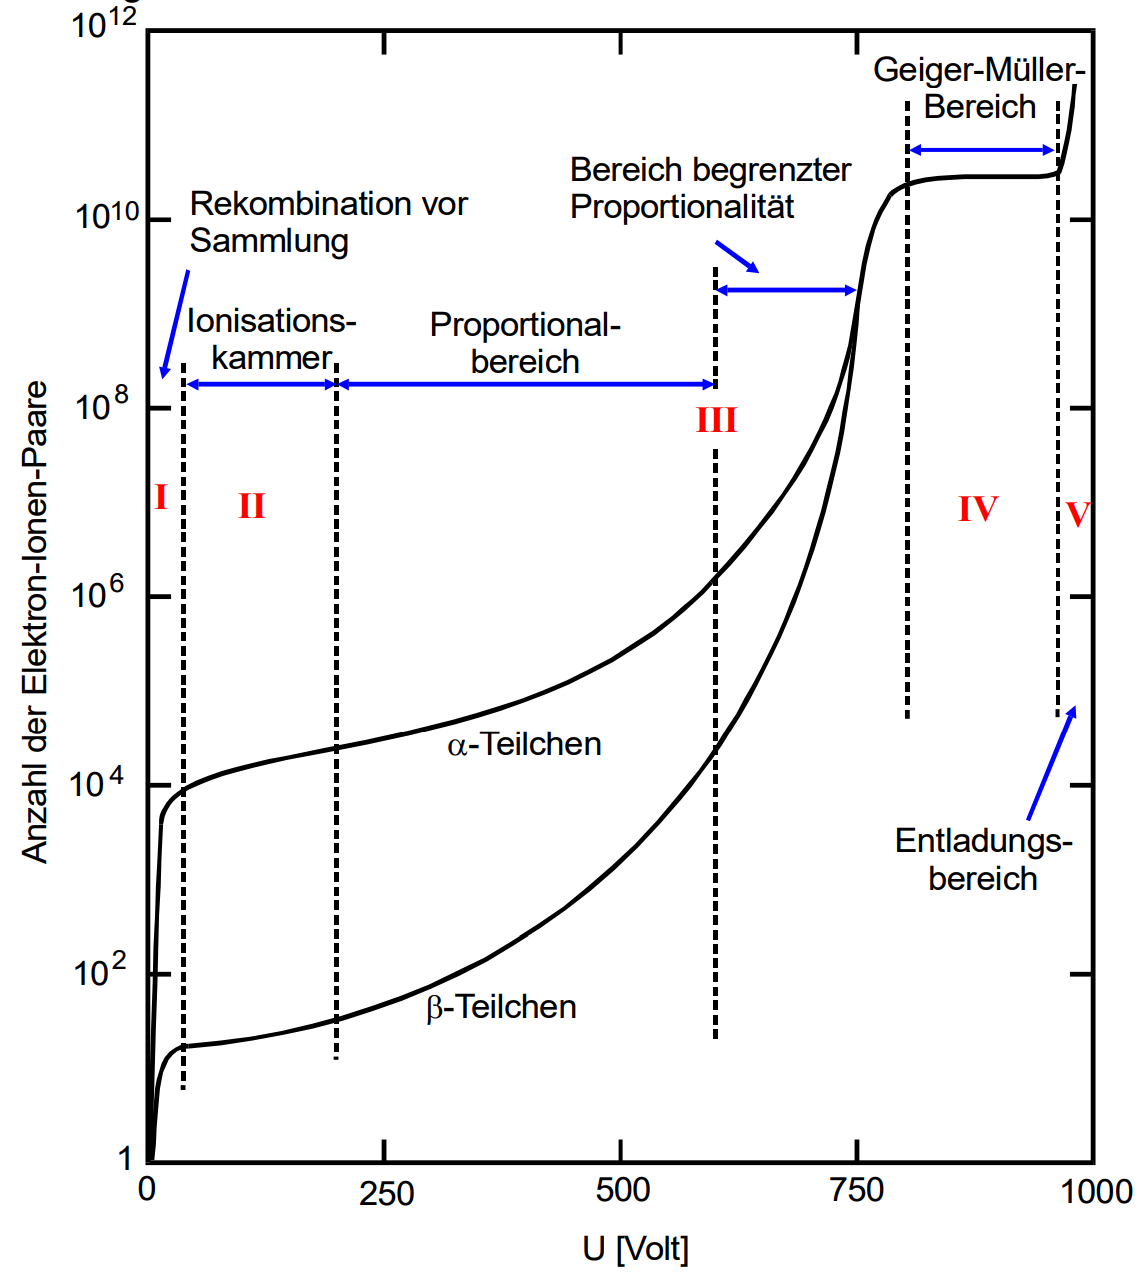
\includegraphics[width=0.3\textwidth]{Abbildungen/Abb_2.png}
    \caption{Arten der Prozesse in Abhängigkeit der angelegten Spannung und Anzahl der Elektron-Ionen-Paare.\cite{V703}}
    \label{fig:Abb_2}
\end{figure}
Daraus ergibt sich, dass in Bereich I nur ein kleiner Anteil der Elektronen den Draht erreicht,
wobei alle weiteren durch vorherige Rekombinationsereignisse verloren gehen. Dieser Bereich wird
Rekombination vor Sammlung genannt. \\
Im nächsten Bereich, Bereich II, ist die Wahrscheinlichkeit für Rekombinationsprozesse geringer und 
nahezu alle erzeugten Elektronen erreichen den Draht. Dieser Bereich wird Ionisationskammer
genannt, weil der Ionisationsstrom im Zählrohr proportional zur Energie wird.\\
In Bereich III erhalten die frei gewordenen Elektronen, aufgrund der erhöhten Beschleunigungsspannung,
genug Energie um ebenfalls Atome zu ionisieren. Diese Ionisierung wird als Stoßionisation
bezeichnet und führt zu einem Lawineneffekt, auch Townsend-Lawine genannt.
Die Ladung der Teilchen ist so groß, dass sie am Zählrohrdraht messbar wird.
Dieser Bereich wird als Proportionalbereich bezeichnet, weil die Ladung proportional zur Energie 
und zur Intensität ist.\\
In Bereich IV wird die Beschleunigungsspannung weiter erhöht und die Ladung wird unabhängig von der
Primärionisation. Dieser Bereich wird Auslösebereich oder Arbeitsbereich des Geiger-Müller-Zählrohrs
genannt.
Neben der Elektronlawine entstehen außerdem UV-Photonen bei der Anregung von Argon-Atomen.
Diese können sich ausbreiten und die gesammelte Ladung am Zählrohrdraht ist nur noch vom Volumen
des Rohres und der Höhe der Betriebsspannung abhängig. 
Das Zählrohr kann nur noch zur Intensitätsmessung genutzt werden, weil keine Proportionalität zwischen 
Primärionisation und Beschleunigungsspannung existiert.\\
In Bereich V kommt es zu einer unkontrollierten Kettenreaktion von Nachladungen, welche zur Zerstörung des
Zählrohrs führt.

\subsection{Einfluss der positiv geladenen Ionen}
\label{subsec:Einfluss}
Positiv geladenen Ionen besitzen eine höhere Masse und bewegen sich deutlich 
langsamer auf die Kathode zu. Dadurch entsteht ein positiver Ionenschlauch, der die Feldstärke
in der Nähe der Anode herabsetzt, sodass keine Stoßionisation mehr möglich ist. Dies führt 
zu einer gewissen Totzeit des Zählrohrs, in der eintreffende Teilchen nicht registriert werden.
Der Ionenschlauch wird über eine bestimmte Zeit neutralisiert, sodass nach der Totzeit $T$
eine Erholungszeit $T_E$ eintritt, in der die ausgehenden Impulse flacher sind. 
Die Verläufe sind in \autoref{fig:Abb_3} dargestellt.
\begin{figure}[H]
    \centering
    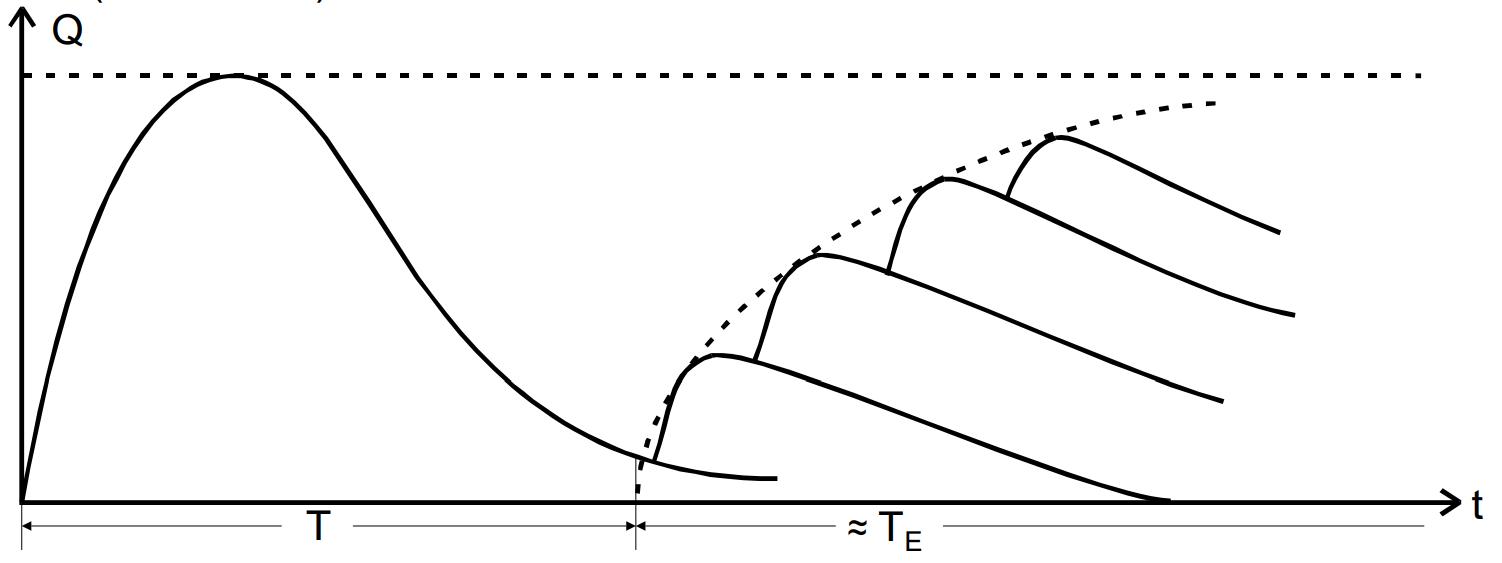
\includegraphics[width=0.3\textwidth]{Abbildungen/Abb_3.png}
    \caption{Charakteristische Verläufe der Totzeit und Erholungszeit des Zählrohrs.\cite{V703}}
    \label{fig:Abb_3}
\end{figure}
Ionen die auf den Zählrohrmantel auftreffen können Elektronen auslösen, weil die Energie,
die durch die Neutralisation frei wird, ausreicht um die Austrittsarbeit für Sekundärelektronen
zu übersteigen. Diese bewegen sich auch zu der Anode und führen zu einer Nachentladung, sodass durch ein eintreffendes
Teilchen zwei oder mehr Ausgangsimpulse entstehen. Die Zeitdifferenz zum Erstimpuls ist größer
als die Totzeit, weswegen die Nachentladungen als reguläre Impulse aufgezeichnet werden. 
Um diese Messunsicherheit auszugleichen, ist im Zählrohrvolumen neben dem Edelgas auch Alkoholdampf.
Dies führt dazu, dass Edelgasionen vor dem Eintreffen an der Kathode mit den Alkoholmolekülen zusammenstoßen
und diese zu Schwingungen anregen, aufgrund der niedrigen Ionisationsenergie.
Durch den Zusammenstoß bleiben die Edelgasatome am Ort des Zusammenstoßes und nur die Alkoholmoleküle wandern zur Kathode
und werden dort neutralisiert. Aufgrund der bereits in Schwingungen umgesetzte Energie reicht die Energie nicht aus 
um weitere Elektronen auszulösen.
Es wird somit nur ein Impuls ausgelöst, wenn tatsächlich ein ionisierendes Teilchen in das Zählrohr fällt.
Dies entspricht nur dem Idealfall.

\subsection{Charakteristik des Zählrohrs}
\label{subsec:Charakteristik}
Im Folgenden wird der Arbeitsbereich des Geiger-Müller-Zählrohrs (Bereich IV in \autoref{fig:Abb_2}) und seine unmittelbare Umgebung genauer betrachtet.
\autoref{fig:Abb_4} zeigt, dass sich beim Auftragen der Teilchenzahl $N$ gegen die angelegte Spannung $U$  die Charakteristik des Zählrohrs ergibt.
\begin{figure}[H]
    \centering
    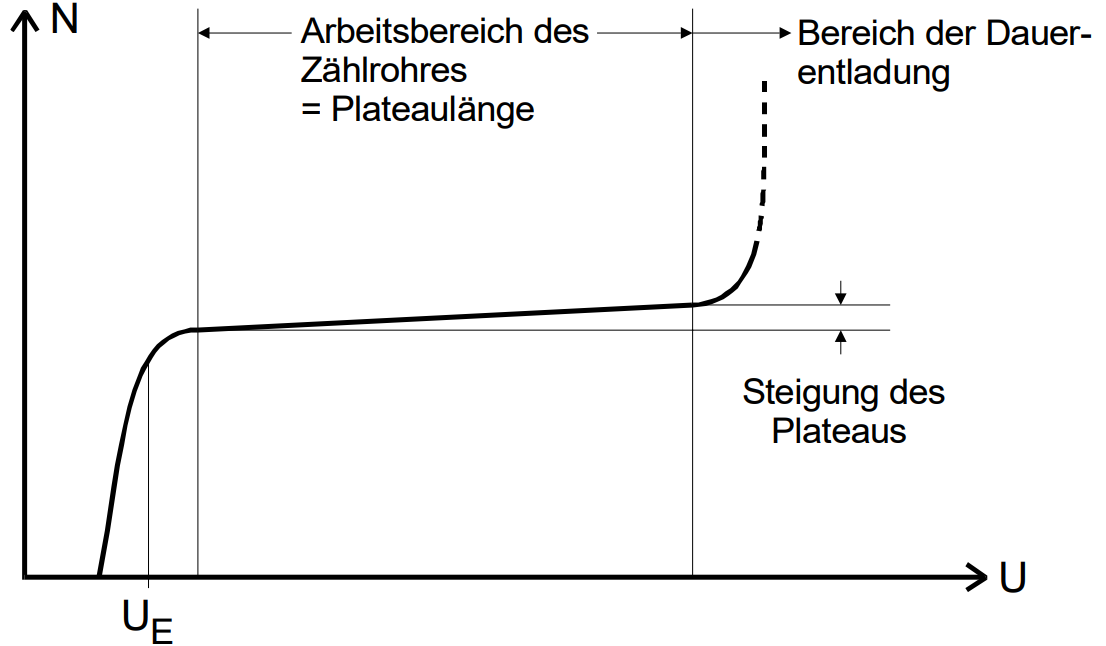
\includegraphics[width=0.3\textwidth]{Abbildungen/Abb_4.png}
    \caption{Charakteristisches Plateau eines Zählrohrs.\cite{V703}}
    \label{fig:Abb_4}
\end{figure}
Dabei ist $U_E$ der Startpunkt des Auslösebereichs , welcher aus einem linearen Teil, dem Plateau besteht.
Unter idealen Bedingungen besitzt das Plateau keine Steigung, jedoch gibt es immer eine Nachentladung und somit eine 
Steigung. Je niedriger die Steigung, desto hochqualitativer ist das Zählrohr.
Am Ende des Plateaus kommt es zu einer selbständigen Gasentladung, einer Kettenreaktion, die nicht zu kontrollieren ist.
Dieser Bereich der Beschleunigungsspannung sollte nicht erreicht werden, um die Zerstörung des Zählrohrs zu verhindern.

\subsection{Ansprechvermögen des Zählrohrs}
\label{subsec:Ansprechvermögen}
Das Ansprechvermögen ist die Wahrscheinlichkeit mit der ein einfallendes Teilchen einen Ausgangsimpuls auslöst.
Die $\alpha$- und $\beta$-Strahlungen besitzen ein Ansprechvermögen von $\qty{100}{\percent}$. Die Öffnung wird mit einer 
dünnen Mylar-Folie ausgestattet, damit die Strahlung in das Zählrohrvolumen eindringen kann. Diese Folie besteht aus Atomen
geringer Ordnungszahl, durch das selbst $\alpha$-Teilchen dringen können. Photonen, also $\gamma$-Strahlung, können
mit diesem Versuchsaufbau nicht detektiert werden. Diese besitzen ein Ansprechvermögen von $\qty{1}{\percent}$. Um das Prinzip des 
Geiger-Müller-Zählrohrs trotzdem verwenden zu können, muss ein schweres Edelgas wie Xenon als Füllgas verwendet werden.
